\chapter{INTRODUÇÃO}

O crescimento das pesquisas em finanças quantitativas nas universidades brasileiras tem evidenciado a necessidade de infraestruturas de dados robustas e de alto desempenho. No âmbito do projeto \textbf{Análise de Séries Financeiras}, vinculado ao Laboratório de Tecnologias Inovadoras (LTI) da Universidade Federal do Ceará (UFC), \textit{campus} de Russas, pesquisadores e estudantes necessitam de acesso contínuo e confiável a séries temporais de ativos financeiros — cotações históricas e em tempo real de ações, câmbio e outros instrumentos — para viabilizar pesquisas de modelos quantitativos. Além disso, a obtenção de dados de maneira \textit{headless} (sem interface gráfica interativa) torna-se uma exigência em projetos com uma quantidade significativa de membros.

A ausência de uma infraestrutura centralizada impõe custos operacionais substanciais. Individualmente, cada pesquisador precisaria implementar conexões com provedores de dados externos (\textit{web-sockets}, dependências de bibliotecas, etc.), gerenciar credenciais de corretoras, lidar com falhas de conectividade e manter códigos de coleta que fogem do escopo de sua especialidade científica. Em face dessa problemática, estabelecemos a seguinte questão norteadora para o presente trabalho: \textit{Como fornecer serviços de software de séries temporais para o LTI de forma centralizada, garantindo alto desempenho, consistência dos dados, alta disponibilidade do serviço e controle de acesso seguro, sem que cada pesquisador precise implementar suas próprias integrações?} Traçamos essa pergunta-problema visando como resposta uma solução-produto de potencial econômico real, isto é, com valor percebido por pessoas interessadas na área quantitativa do mercado financeiro.

Para solucionar essa questão, surgiu a necessidade de desenvolver uma plataforma que atendesse às demandas de discentes e docentes quanto ao acesso a dados históricos e em tempo real. Essas demandas estruturam-se em requisitos funcionais (obtenção de cotações, volume transacionado, ordens agendadas) e não funcionais (alto desempenho, consistência dos dados mantida sob alta taxa de ingestão, mecanismos iniciais de disponibilidade do serviço e controle de acesso granular). A partir dessa perspectiva, iniciamos a concepção de um núcleo \textit{headless} e centralizado de dados financeiros.

Diante disso, desenhou-se um "ponto de partida" que consistia, inicialmente, em uma simples API de séries temporais, mas que evoluiu, a nível de produto, para um ecossistema de serviços de dados financeiros. Tal afirmação justifica-se pelo fato de que a solução proposta iniciou-se como (1) um projeto técnico restrito a um núcleo de dados (qDATA), expandiu-se para (2) um escopo de serviço de software completo (abrangendo foco em disponibilidade, documentação, gerenciamento de permissões e \textit{Service Level Agreement}) e, por fim, (3) influenciou a concepção de outros serviços complementares. Portanto, o escopo do presente trabalho é radial e expansivo, perpassando o \textit{design} arquitetural, gerenciamento do projeto e \textit{design} de produtos.

\begin{figure}[htb]
    \centering
    \caption{Serviços e seus respectivos bancos de dados independentes.}
    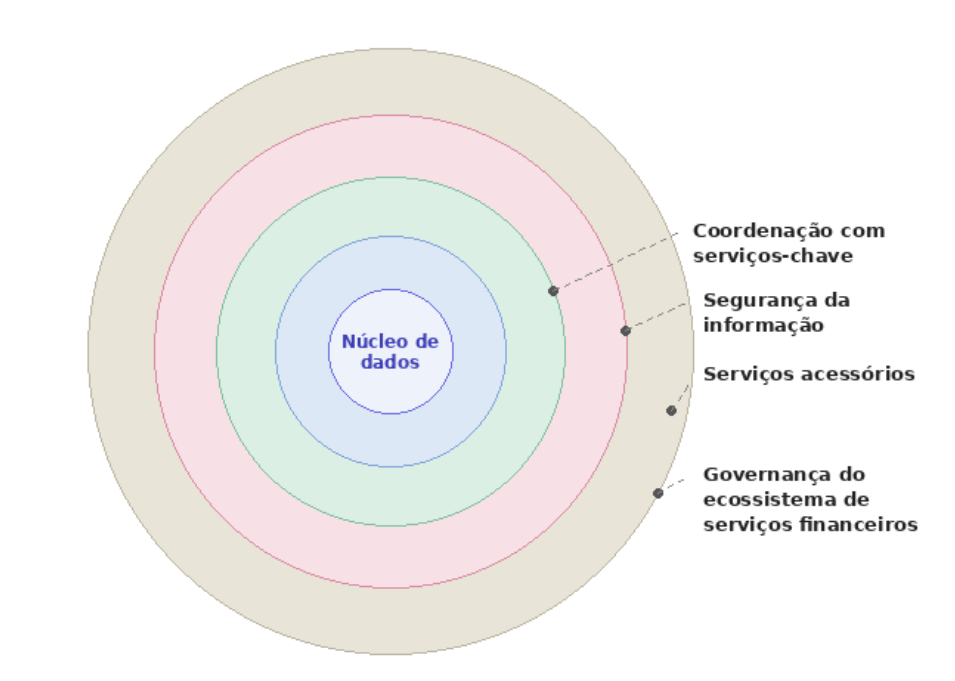
\includegraphics[width=\textwidth]{assets/figura_1_bancos_independentes.png}
    \label{fig:bancos_independentes}
\end{figure}

Para concretizar essa visão, pensamos um núcleo de armazenamento e distribuição baseada em \textit{containers} Docker. A etapa de aquisição de dados, implementada de forma independente por Evamberto Oliveira, executa o \textit{MetaTrader 5} integrado a provedores externos, como as corretoras Rico, XP e Inter. Esses contêineres de extração (mt5BRIDGE) enviam os dados dos ativos para um canal da API de armazenamento do qDATA, que os persiste no banco de dados. Toda a ingestão ocorre via Representational State Transfer (REST)/HTTPS, justificável pelo fluxo relativamente baixo de entrada de dados, o que evidencia a coordenação necessária entre o mt5BRIDGE e o qDATA.

A persistência no qDATA é gerenciada por um banco de dados PostgreSQL com estratégia de \textit{Upsert} (Update + Insert). Essa abordagem previne duplicidades e mantém a consistência das informações mesmo sob alta taxa de ingestão simultânea. Ademais, o armazenamento é otimizado para séries temporais por meio do uso de hyper-tabelas da extensão TimeScale.

No que tange à distribuição técnica dos dados, o protocolo \textit{gRPC Remote Procedure Call} (gRPC) permite o estabelecimento de conexões contínuas (com sessão) e uma obtenção mais rápida, sendo útil em consultas massivas, como o resgate de dados correspondentes a um ano inteiro. Contudo, visando complementar e facilitar essa distribuição, implementou-se também uma interface HTTPS/2. Essa segunda opção foi projetada para que a conexão com a API pudesse ser realizada de forma mais ágil pelos usuários (pesquisadores e desenvolvedores), uma vez que o uso de HTTPS apresenta uma curva de aprendizado substancialmente menor e um \textit{overhead} de desenvolvimento reduzido.

À medida que a ferramenta avançou em produção, membros do projeto passaram a utilizá-la como base para construir serviços quantitativos auxiliares, tais como cálculos de correlações com \textit{bootstrapping}, experimentos em Python de trabalhos teóricos conduzidos no projeto, e rotinas de identificação de anomalias. Esse cenário reforça o desenho de um ecossistema coeso de serviços e análises de apoio.

Por fim, cabe ressaltar que a plataforma qDATA é uma ferramenta de uso estritamente interno ao Laboratório de Tecnologias Inovadoras (LTI) e à comunidade de pesquisa da Universidade Federal do Ceará. Ela não configura um serviço comercial de distribuição de dados de mercado para terceiros externos. Assim, estabelecemos uma rigorosa política de não revenda, não sublicenciamento e não disponibilização pública dos dados obtidos. Essa segurança reflete-se no gerenciamento granular de permissões de acesso em um banco de dados específico. A implantação de contêineres individuais para aquisição de dados será, futuramente, discutida com o responsável pelo mt5BRIDGE.

A arquitetura do ecossistema de microsserviços promove o princípio de \textbf{Separação de Responsabilidades} (\textit{Separation of Concerns}): o qDATA concentra-se exclusivamente no fornecimento dos dados como serviço compartilhado, enquanto as ferramentas dos pesquisadores — painéis analíticos, algoritmos de ordens de \textit{trading} e modelos estatísticos — focam em suas lógicas específicas. Isso elimina acoplamentos indesejados e permite que diferentes membros do LTI e projetos da UFC utilizem essa infraestrutura de dados sem redundâncias.

\begin{figure}[htb]
    \centering
    \caption{Visão geral da arquitetura: Ingestão distribuída e distribuição segura de dados financeiros.}
    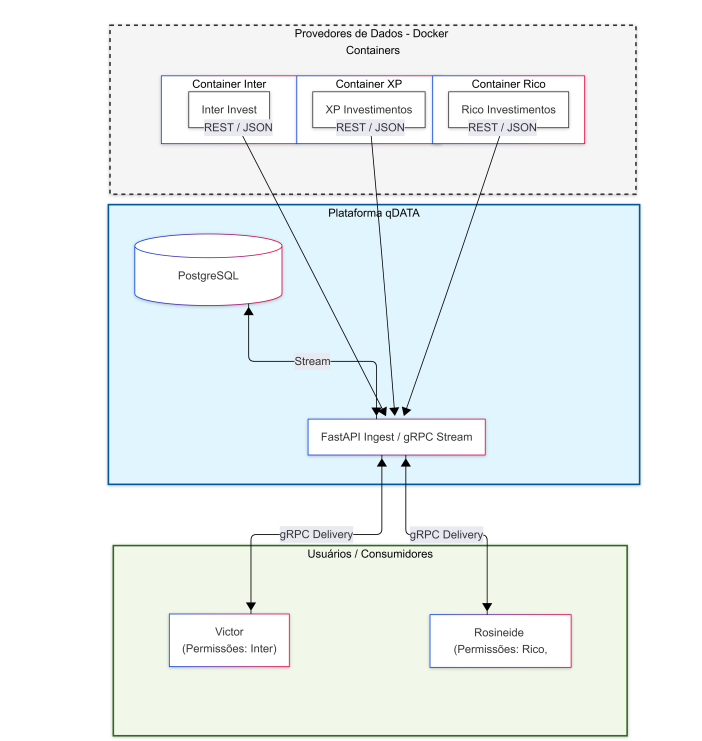
\includegraphics[width=\textwidth]{assets/figura_2_visao_arquitetura.png}
    \label{fig:visao_arquitetura}
\end{figure}

Deve-se observar, no entanto, que o uso em outros projetos requer, por questões legais e de governança, a execução de uma nova instância isolada do sistema, haja vista as restrições à distribuição. Nesse contexto de separação de responsabilidades, a execução de ordens de compra e venda, por exemplo, permanece uma tarefa local e autônoma de cada ferramenta consumidora, sem interferência direta com a camada de ingestão remota ou de distribuição de dados. Tanto por questões legais quanto de engenharia de software, decidiu-se consolidar o ecossistema sob o escopo do \textit{LTI FinHub}.

O acesso à plataforma é protegido por autenticação baseada em \textit{JSON Web Token} (JWT) integrada ao Supabase, viabilizando um controle de acesso granular por perfil de usuário e por provedor de dados. Dessa forma, o trabalho aqui apresentado descreve a concepção, a arquitetura e a implementação dessa infraestrutura de dados, avaliando sua contribuição para as atividades do LTI e a viabilidade do uso da ferramenta em outros projetos da UFC.

\begin{figure}[htb]
    \centering
    \caption{Diagrama de consumo e execução: Autonomia dos pesquisadores e separação de responsabilidades.}
    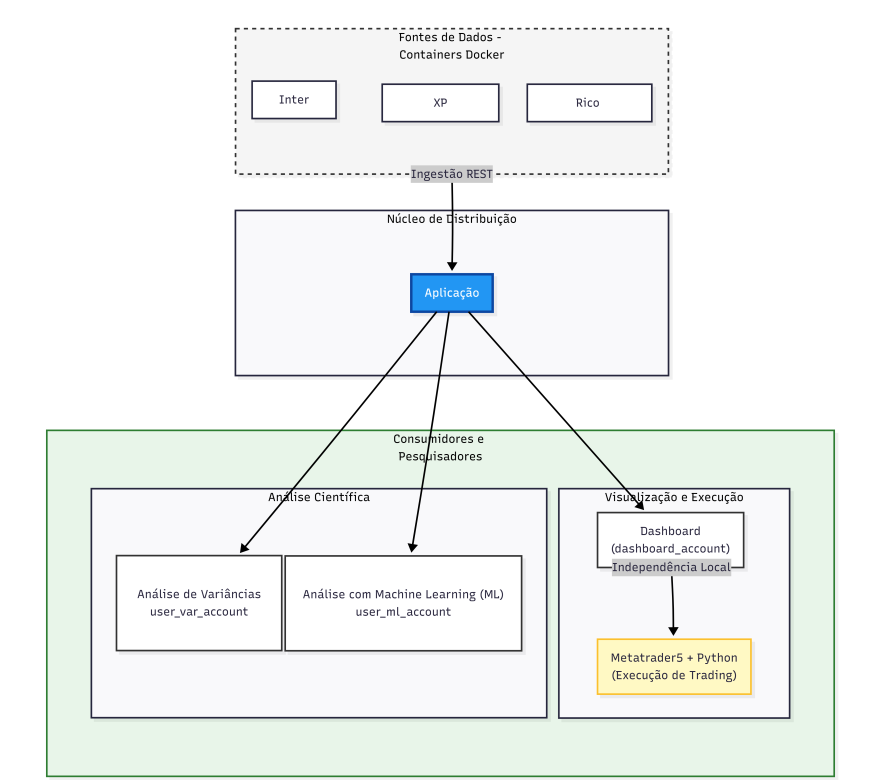
\includegraphics[width=\textwidth]{assets/figura_3_autonomia_pesquisadores.png}
    \label{fig:autonomia_pesquisadores}
\end{figure}

\section{Escopo}

A plataforma qDATA abrange a ingestão de dados de corretoras selecionadas, o armazenamento e a distribuição desses dados para consumidores internos do grupo de pesquisa LTI, com foco no projeto \textit{Análise de Séries Financeiras}. Dentro do escopo técnico estão a comunicação com um software de aquisição de barras \textit{Open, High, Low, Close} (OHLC), o armazenamento otimizado com hyper-tabelas através do TimeScale — o que viabiliza a entrega de dados em alta velocidade aos consumidores autorizados — e a disponibilização desses dados via HTTPS, visando cenários que exigem praticidade e agilidade no desenvolvimento de aplicações.

Ao longo deste trabalho, também são analisadas as políticas de acesso a dados, o registro e ativação de usuários, o gerenciamento de contas do projeto e outras questões de segurança que impactam diretamente a ferramenta qDATA e o ecossistema como um todo. Assim, partindo da ferramenta qDATA como elemento central, o escopo se expande radialmente para uma visão arquitetural mais ampla, englobando o apoio à governança de TI do projeto \textit{LTI Finanças}.

\begin{figure}[htb]
    \centering
    \caption{Demandas do núcleo de dados.}
    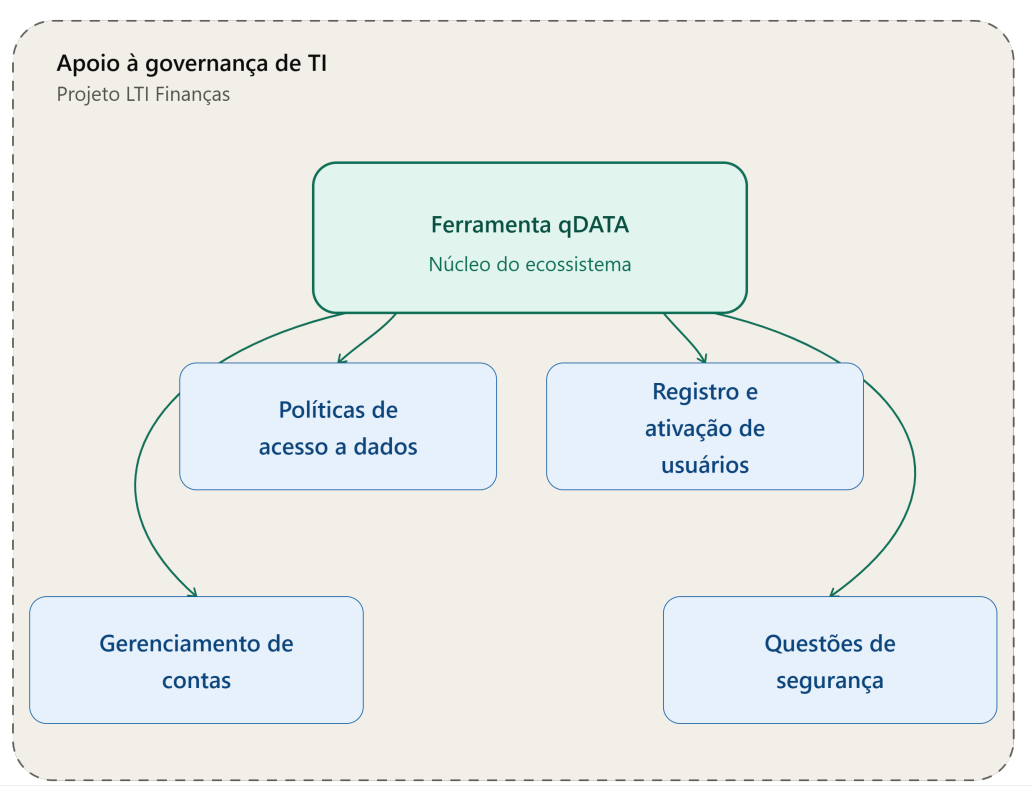
\includegraphics[width=\textwidth]{assets/figura_4_demandas_nucleo.png}
    \label{fig:demandas_nucleo}
\end{figure}

Por outro lado, estão categoricamente fora do escopo desta plataforma: a execução de ordens de compra e venda nas corretoras, a gestão de risco financeiro e o desenvolvimento de interfaces de \textit{trading} para usuários finais. O qDATA atua exclusivamente como infraestrutura de dados compartilhada, cabendo à lógica de análise e negociação permanecer sob a estrita responsabilidade de cada ferramenta ou pesquisador consumidor.

\section{Objetivos}

\subsection{Objetivo Geral}

Projetar e implementar uma plataforma de dados financeiros centralizada e orientada à disponibilidade para o projeto \textit{Análise de Séries Financeiras} do LTI.

\subsection{Objetivos Específicos}

\begin{itemize}
    \item Integrar a plataforma com os \textit{containers} Docker de aquisição de dados do MetaTrader 5 (MT5), os quais operam em ambiente Linux utilizando Wine;
    \item Desenvolver o núcleo de ingestão e armazenamento de dados empregando o \textit{framework} FastAPI e o banco de dados PostgreSQL, mediado por protocolo HTTPS REST;
    \item Implementar serviços de distribuição de dados aos consumidores utilizando o protocolo gRPC;
    \item Disponibilizar uma interface HTTPS análoga ao serviço gRPC, provendo \textit{endpoints} mais amigáveis e flexíveis para desenvolvedores iniciantes ou colaboradores que priorizam agilidade de prototipagem;
    \item Integrar a arquitetura a um sistema de autenticação e autorização via Supabase e JWT, viabilizando um controle de acesso granular que diferencia permissões de leitura e gravação através de um atributo de modo de usuário;
    \item Estabelecer mecanismos iniciais para a garantia de disponibilidade, abrangendo a implementação de testes unitários (via \texttt{pytest}) e o planejamento de fluxos de integração contínua (GitHub Actions), que utilizam estes testes.
    \item Implementar um ambiente de \textit{staging} em nosso servidor
    \item Validar a robustez da plataforma com consumidores reais do LTI por meio da alimentação do \textit{dashboard} analítico;
    \item Comparar o desempenho das interfaces de distribuição (gRPC, gRPC-Web e HTTPS) em termos de latência e consumo de banda, gerando histogramas para avaliação da variância métrica;
    \item Documentar formalmente as políticas de controle de acesso e versionamento como prática basilar de governança de TI;
    \item Analisar e definir as restrições de \textit{compliance} pertinentes ao uso e à distribuição interna dos dados financeiros coletados.
\end{itemize}

\section{Organização do Trabalho}

Este trabalho está organizado em seis capítulos, incluindo esta introdução. O Capítulo 2 aborda a fundamentação teórica que dá suporte às decisões de \textit{design} e às tecnologias empregadas na plataforma. O Capítulo 3 descreve, de modo pragmático, a metodologia adotada para o desenvolvimento do projeto. O Capítulo 4 apresenta o cronograma das atividades. O Capítulo 5 detalha os resultados técnicos, organizacionais e de adoção obtidos ao longo do trabalho. Por fim, o Capítulo 6 traz a conclusão, delineando as considerações finais e os possíveis trabalhos futuros.
